\setAuthor{}
\setRound{lõppvoor}
\setYear{2019}
\setNumber{G 5}
\setDifficulty{5}
\setTopic{TODO}

\prob{Jääkeegel}
\begin{wrapfigure}{r}{0.38\textwidth}
  \vspace{-25pt}
  \begin{center}
    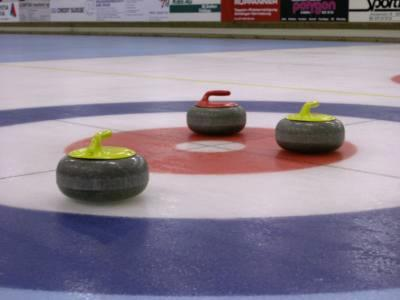
\includegraphics[width=0.4\textwidth]{2019-v3g-05-yl.jpg}
    % Pildi allikas Wikimedia Commons https://upload.wikimedia.org/wikipedia/commons/4/4f/Curling_stones.jpg
  \end{center}
  \vspace{-20pt}
\end{wrapfigure}

Jääkeegel ehk kurling on talispordimäng, mille eesmärgiks on enda meeskonna kivide libistamine jääväljakule märgitud märklaua keskkohale võimalikult lähedale. Sealjuures on lubatud enda kividega vastase kivisid eemale tõugata. Vaatamegi olukorda, kus vastasel on õnnestunud üks kivi täpselt märklaua keskele libistada. Kui suure kiirusega $v_0$ peaks oma kiviga vastase kivi tabama, et pärast vastase kivi eemaletõukamist jääks see ise täpselt märklaua keskele? Jääkeeglikivid on võrdse massiga ning läbimõõduga $D=\SI{29}{cm}$. Hõõrdetegur jää ja kivide vahel on $\mu = \num{0.02}$ ning kividevahelisel põrkel muundub soojuseks $\eta=40\%$ esialgsest kineetilisest energiast. Raskuskiirendus $g=\SI{9.8}{m/s^2}$.


\hint

\solu
Esmalt veendume selles, et esialgu liikuva kivi märklaua keskele jõudmiseks peab kivide vahel toimuma tsentraalne otsepõrge. Oletame vastuväiteliselt, et liikuva kivi trajektoori pikendus ei läbi enne põrget seisva kivi massikeset, vaid möödub sellest näiteks paremalt poolt (liikumise sihis vaadatuna). Kuna kivide ristlõiked on ringikujulised ja eeldame, et kivi massikese asub ringi keskel, siis mõjuvad kivide vahel põrke ajal jõud piki nende massikeskmeid ühendavat sirget. Jagades liikumatu kivi poolt liikuvale kivile avaldatava jõu kaheks komponendiks, millest üks on piki kivi esialgset trajektoori ja teine sellega risti, näeme et jõu ristikomponent on suunatud liikumise sihist paremale. Seega pöördub liikuva kivi trajektoor põrke tulemusel veel rohkem paremale ja ei saa läbida märklaua keskpunkti. Järelikult peab ülesande tingimuste täitmiseks toimuma tsentraalne otsepõrge ja saame järgnevalt olukorda vaadelda ühemõõtmelisena.

Märklaua keskele jõudmiseks peab esialgu liikuv kivi pärast põrget teatud kiirusega edasi liikuma ja seejärel jääga hõõrdumise tõttu seisma jääma. Tähistame kiirused: $v_0$ ja $v$ -- esialgu liikuva kivi kiirus enne ja pärast põrget ning $u$ -- esialgu seisva kivi kiirus pärast põrget. Impulsi jäävuse seadusest:
\begin{equation}
mv_0 = mv + mu,
\end{equation}
kus $m$ on kivi mass, mis nagu näha välja taandub. Samuti saame kirjutada energia jäävuse seaduse
\begin{equation}
\left(1-\eta\right)\frac{mv_0^2}{2} = \frac{mv^2}{2} + \frac{mu^2}{2},
\end{equation}
kus $\eta = \num{0.4}$ on põrkel kaduma läinud energia osakaal.

Kiiruse $v$ jaoks kehtib tingimus
\begin{equation}
\frac{mv^2}{2} = \mu mgs,
\end{equation}
ehk esialgu liikuva kivi kineetiline energia pärast põrget on võrdne hõõrdejõu tööga kivi seismajäämisel. Põrke hetkel on esialgu liikuva kivi keskkoha kaugus märklauast võrdne kivi läbimõõduga ehk $s = D$ ja $v = \sqrt{2\mu gD}$.

Kiiruse $v_0$ leidmiseks avaldame impulsi jäävuse seadusest $u = v_0 - v$ ja asetame selle energia jäävuse avaldisse:
\begin{equation}
\left( 1 - \eta \right)v_0^2 = v^2 + \left(v_0 - v\right)^2, 
\end{equation}
millest
\begin{equation}
\eta v_0^2 - 2v_0 v + 2v^2 = 0.
\end{equation}
Saadud ruutvõrrandi lahend on
\begin{equation}
v_0 =  \frac{v\left( 1 \pm \sqrt{1-2\eta} \right)}{\eta}
\end{equation}
ehk kasutades eelnevalt leitud $v$ avaldist, saame
\begin{equation}
v_0 =  \frac{\sqrt{2\mu gD}\left( 1 \pm \sqrt{1-2\eta} \right)}{\eta}.
\end{equation}
Vastavalt märgile ruutvõrrandi lahendi valemis saaksime kiirusteks

\begin{center}
\begin{tabular}{|c|c|c|}
\hline 
 & $+$ & $-$ \\ 
\hline 
$v_0$ & \SI{1.22}{m/s} & \SI{0.47}{m/s} \\ 
\hline 
$v$ & \SI{0.34}{m/s} & \SI{0.34}{m/s} \\ 
\hline 
$u$ & \SI{0.88}{m/s} & \SI{0.13}{m/s} \\ 
\hline 
\end{tabular}
\end{center}

Kuna kivid ei saa pärast põrget üksteisest läbi minna, siis peab kehtima $u > v$ ja füüsikaliselt sobib ainult pluss-märgiga lahend ehk kivi kiirus enne põrget on $v_0 = \SI{1.2}{m/s}$.
\probend